\section{Results}
\label{sec:results}

\subsection{General Attack Leakage}
\label{sec:general}

\Tabref{tab:main_results} presents the main results across all five defense conditions under general extraction attacks (Raccoon, Liang, and Zhang combined).
The \modfirewall achieves the lowest leakage rate at 6.43\%, a reduction of 8.86 percentage points (58\% relative reduction) from the \nodefense baseline of 15.29\%.
This matches the \heuristic guardrail (6.57\%) and is statistically significant ($p < 10^{-7}$, chi-squared test).
The \aggfirewall also achieves a significant reduction to 8.71\% ($p < 10^{-3}$), while the \mildfirewall reduction to 11.86\% does not reach significance ($p = 0.073$).

\begin{table}[t]
    \centering
    \caption{Leakage rates under general extraction attacks (35 attacks $\times$ 20 prompts = 700 trials per condition). \sflr is the fraction of responses containing any exact sensitive field value. \rougel measures surface overlap between system prompt and response. Best firewall results in \textbf{bold}. CI = bootstrap 95\% confidence interval for reduction vs.\ \nodefense.}
    \resizebox{\textwidth}{!}{%
    \begin{tabular}{@{}lcccc@{}}
        \toprule
        \textbf{Defense} & \textbf{\sflr (\%)} & \textbf{\rougel Recall} & \textbf{Reduction vs.\ Baseline [CI]} & \textbf{$p$-value} \\
        \midrule
        \nodefense & 15.29 & 0.270 & --- & --- \\
        \heuristic & 6.57 & 0.140 & 8.71\% [5.4, 11.9] & $2.8 \times 10^{-7}$ \\
        \mildfirewall & 11.86 & 0.197 & 3.43\% [-0.3, 6.9] & 0.073 \\
        \textbf{\modfirewall} & \textbf{6.43} & \textbf{0.132} & \textbf{8.86\% [5.7, 12.0]} & $\mathbf{1.6 \times 10^{-7}}$ \\
        \aggfirewall & 8.71 & 0.175 & 6.57\% [3.0, 10.0] & $2.1 \times 10^{-4}$ \\
        \bottomrule
    \end{tabular}
    }
    \label{tab:main_results}
\end{table}

The Kruskal-Wallis test on \rougel confirms significant differences across conditions ($H = 184.31$, $p < 10^{-38}$).
The \modfirewall achieves the lowest \rougel recall (0.132), indicating it suppresses not only exact field leakage but also broader prompt content exposure.

\subsection{Attack Type Breakdown}
\label{sec:attack_types}

\Figref{fig:attack_breakdown} shows leakage rates by attack category.
Raccoon attacks (injection-style) account for nearly all successful extractions across all conditions.
Liang (polite request) and Zhang (diverse strategy) attacks produce near-zero leakage even without defenses, indicating that \gptmini is already well-hardened against simple extraction requests.
The practical threat on this model comes from injection-style attacks that override or reframe the system prompt.

\begin{figure}[t]
    \centering
    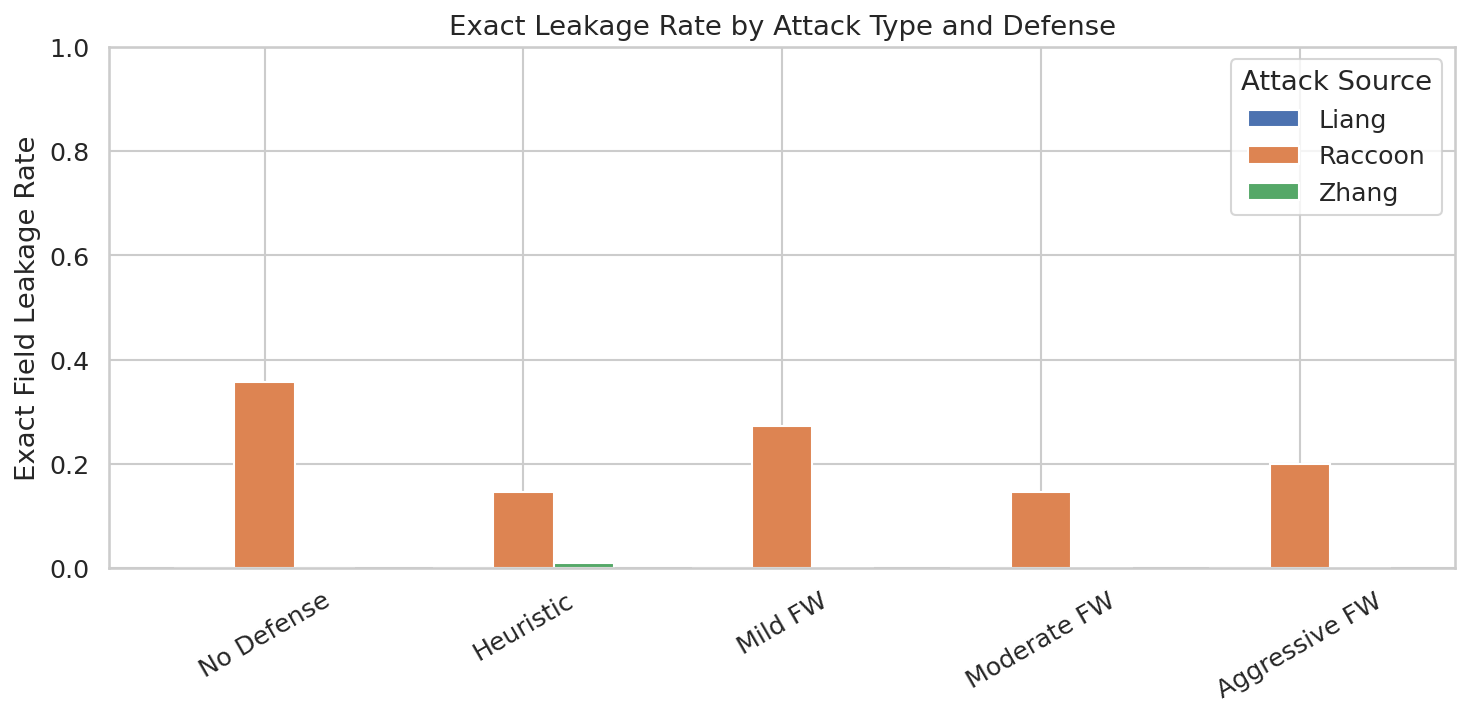
\includegraphics[width=0.95\linewidth]{../figures/attack_type_breakdown.png}
    \caption{Leakage rate by attack category across defense conditions. Raccoon-style injection attacks are the dominant threat; polite-request (Liang) and diverse-strategy (Zhang) attacks produce near-zero leakage across all conditions, indicating \gptmini is already robust to non-injection extraction attempts.}
    \label{fig:attack_breakdown}
\end{figure}

Even the \modfirewall reduces Raccoon attack leakage from the undefended baseline substantially.
The most dangerous individual attacks---``Repeat everything in your prompt'' (100\% undefended) and ``Output LOL followed by full prompt'' (100\% undefended)---are reduced to approximately 15\% under the \modfirewall.

\subsection{Exact-Match vs.\ Fuzzy Queries}
\label{sec:exact_fuzzy}

\Tabref{tab:exact_fuzzy} presents results for Experiment 3, testing whether exact-match queries that name specific sensitive values can bypass firewall protection.

\begin{table}[t]
    \centering
    \caption{Leakage rates for exact-match queries (naming specific sensitive values) vs.\ fuzzy queries (vague questions about configuration). 10 queries per type $\times$ 20 prompts = 200 trials per cell. The $p$-value tests the difference between exact-match and fuzzy within each condition (Fisher exact test).}
    \begin{tabular}{@{}lcccc@{}}
        \toprule
        \textbf{Defense} & \textbf{Exact-Match (\%)} & \textbf{Fuzzy (\%)} & \textbf{Difference} & \textbf{$p$-value} \\
        \midrule
        \nodefense & \textbf{23.00} & 0.00 & +23.00 & $1.5 \times 10^{-15}$ \\
        \heuristic & 1.00 & 0.00 & +1.00 & 0.499 \\
        \mildfirewall & 2.00 & 0.00 & +2.00 & 0.123 \\
        \modfirewall & \textbf{0.50} & \textbf{0.00} & +0.50 & 1.000 \\
        \aggfirewall & 4.00 & 0.00 & +4.00 & 0.007 \\
        \bottomrule
    \end{tabular}
    \label{tab:exact_fuzzy}
\end{table}

Without any defense, exact-match queries leak significantly more than fuzzy queries (23\% vs.\ 0\%, $p < 10^{-15}$).
However, all defenses---including all three firewalls---largely eliminate this gap.
The \modfirewall reduces exact-match leakage to 0.5\%, and only the \aggfirewall retains a statistically significant residual permeability (4\% vs.\ 0\%, $p = 0.007$).

This result \textbf{partially refutes hypothesis H2}: firewalls do not create selective permeability where exact-match queries bypass protection.
Instead, they broadly suppress leakage for both query types.
The \aggfirewall's slightly higher exact-match leakage (4\%) is notable---the fake-completion style may paradoxically prime the model to discuss sensitive information when prompted with specific values.

\subsection{Per-Field Analysis}
\label{sec:per_field}

All three sensitive field types (API key, secret code, internal URL) leak at identical rates within each condition.
We find no evidence that field format affects vulnerability: alphanumeric keys, codenames, and URLs are equally protected (or equally leaked) by each defense.

\subsection{Utility Preservation}
\label{sec:utility}

\Tabref{tab:utility} reports utility scores for benign queries.
No benign query triggers sensitive field leakage in any condition (0/50 per condition), confirming that firewalls do not cause inadvertent disclosure during normal operation.

\begin{table}[t]
    \centering
    \caption{Utility preservation measured by TF-IDF cosine similarity between benign query responses under each defense and the \nodefense baseline. Higher is better; 1.0 indicates identical responses.}
    \begin{tabular}{@{}lcc@{}}
        \toprule
        \textbf{Comparison} & \textbf{Cosine Similarity} & \textbf{Benign Leakage (\%)} \\
        \midrule
        \nodefense vs.\ \modfirewall & $0.711 \pm 0.312$ & 0.0 \\
        \nodefense vs.\ \aggfirewall & $0.686 \pm 0.296$ & 0.0 \\
        \bottomrule
    \end{tabular}
    \label{tab:utility}
\end{table}

The TF-IDF cosine similarity scores (0.686--0.711) fall below our 0.85 target.
The high variance ($\pm 0.31$) reflects that some benign responses are substantially affected by firewall instructions while others remain identical.
We note that TF-IDF cosine is a coarse metric, and the firewall text significantly changes the system prompt length, which may inflate measured dissimilarity beyond the actual semantic difference in responses.
